\chapter{Application à l'analyse descriptive d'un grand corpus}
\label{chap:demo}
Ce chapitre décrit des résultats d'analyses statistiques observés lors de l'application de la chaîne proposée (Figure \ref{fig:intro:pipeline-globale}) sur un corpus formé de la base CAPP de la \citet{dila2019capp} (+65k XML sur 1997-2019),  une base du tribunal de commerce de Paris (300k MS DOC sur ?-?), 500k décisions collectées de Legifrance, et plus de 10k autres documents de cours d'appels. Le module d'extraction d'information (Figure \ref{fig:demo:module-extraction}) est un système qui comprend les modèles développés durant les expérimentations de cette thèse. 
%à CAPP\_20190805-214041.tar.gz et Freemium_capp\_global\_20180315-170000.tar.gz 

%\verb|wget -c --accept='*.tar.gz' -r  ftp://echanges.dila.gouv.fr/CAPP/|

\begin{figure}[!htb]
	\centering 
	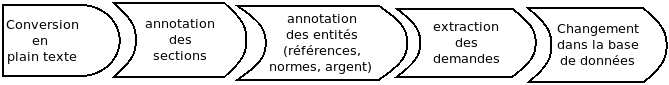
\includegraphics[width=0.8\textwidth]{pipeline-demo.png}
	\caption{Détails du module d'extraction d'information}\label{fig:demo:module-extraction}
\end{figure}

Après extraction, la base de données comprend +65k documents répartis dans l'espace (ville) comme sur la figure \ref{fig:demo:doc-per-city} et dans le temps comme sur la figure \ref{fig:demo:doc-per-year}.

\begin{figure}[ht]
	\centering
	\begin{subfigure}[ht]{0.5\textwidth}
		\centering
		\centering
		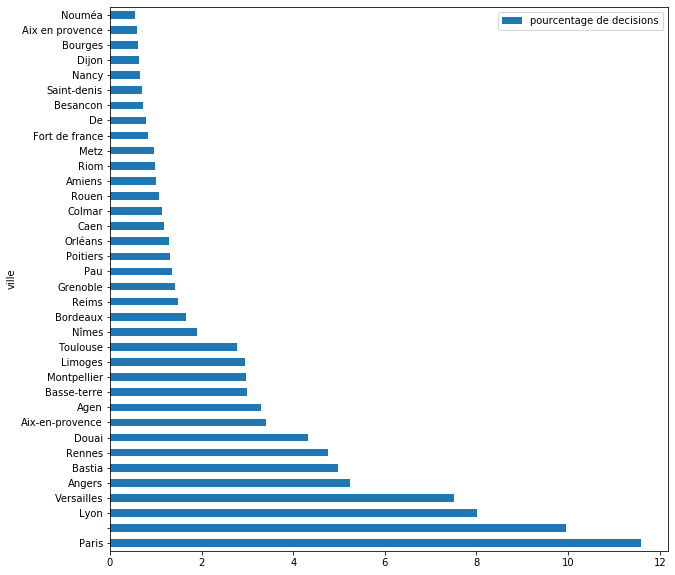
\includegraphics[width=\textwidth]{demo-pourcentage-decision-par-ville.png}
		\caption{Par ville (pourcentage>0)} \label{fig:demo:doc-per-city}
	\end{subfigure} 
	\begin{subfigure}[ht]{0.45\textwidth}
		\centering
		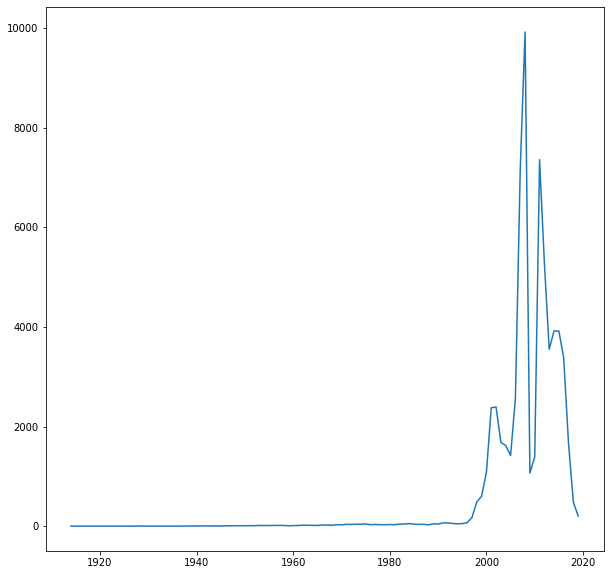
\includegraphics[width=\textwidth]{demo-repartition-decision-par-annee-1900_2019.png}
		\caption{Par an (entre 1900 et 2019)} \label{fig:demo:doc-per-year}
	\end{subfigure}
	\caption{Répartition des décisions} \label{fig:structuration:learning-curves}
\end{figure}


La structuration des données dans la base de données permet de comprendre mieux la jurisprudence à l'aide de graphiques appropriés. Une application de visualisation a notamment été développée suivant les besoins d'un expert juriste par \citet{PRYSIAZHNIUK2017jurisprudence-demo-web}.
Les analyses des sections suivantes sont restreintes aux 5 villes ayant les plus grands nombres de décision: Paris, Lyon, Versailles, Angers, Bastia; sur la période 2000-2019

\subsection{Analyse du sens du résultat}
A partir de la base des données extraites, l'évolution du pourcentage de demandes acceptées  peut être observée sur une courbe. En traçant une telle courbe pour chaque ville il est possible de comparer les villes.
Par exemple, pour les dommages intérêts sur l'article 700 du Code de Procédure Civile (STYX), la Figure \ref{fig:demo:analyse-sens-resultat-styx} compare l'évolution du sens du résultat entre les villes citées précédemment. On remarque que les demandes sont beaucoup plus rejetées qu'acceptées. La courbe du nombre total de demandes doit être associée pour savoir si le pourcentage de succès est considérable\footnote{Pour une année ou une seule demande est extraite et acceptée, le pourcentage est à 100\%, mais ce n'est pas considérable.}.

\begin{figure}[!htb]
	\centering 
	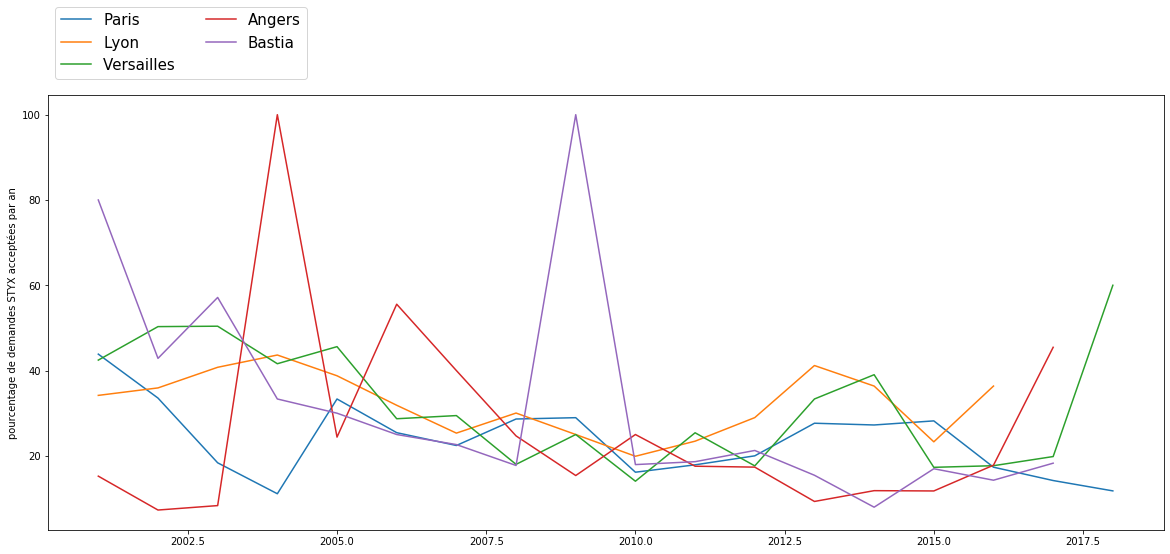
\includegraphics[width=0.9\textwidth]{evolution_sens_resultat_styx.png}
	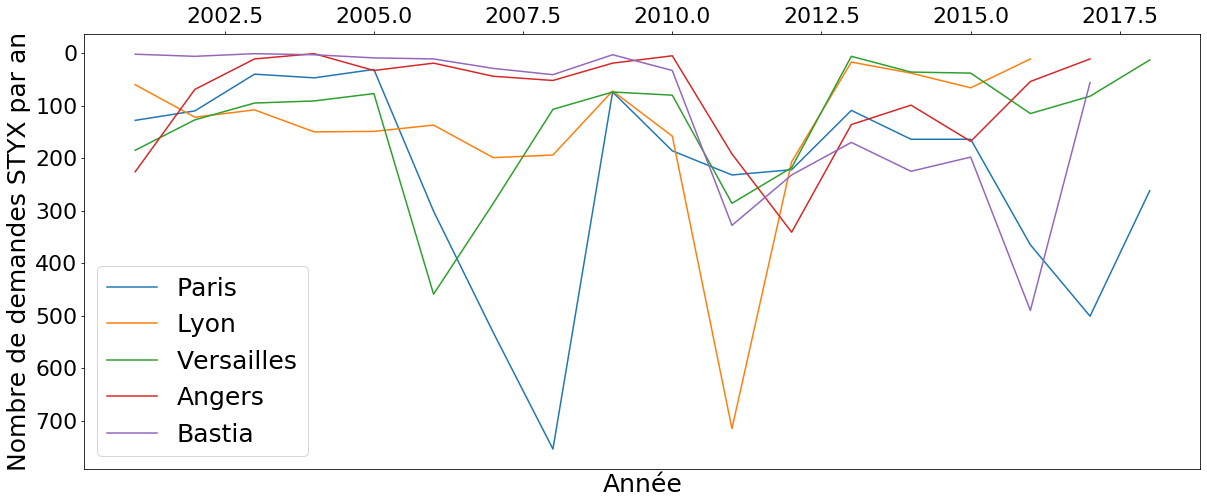
\includegraphics[width=0.9\textwidth]{evolution_nbdmd_styx.png}
	\caption{Evolution du sens du résultat des demandes STYX dans le temps à Paris, Lyon, Versailles, Angers, Bastia.}\label{fig:demo:analyse-sens-resultat-styx}
\end{figure}

La visualisation par l'application de \citet{PRYSIAZHNIUK2017jurisprudence-demo-web} permet de comparer les villes en fonction de l'épaisseur des branches d'arbre (Figure \ref{label})

\subsection{Analyse des quanta}
,bkjlihio
\subsubsection{Evolution dans le temps}
\subsubsection{Différence dans l'espace}
\subsubsection{Quantum demandé vs. quantum accordé}



\section{Conclusion}
\label{sec:demo:conclusion}
hgfgh
lkhk